\section{Analysis of a single dataset --- starting from ``scratch''}
\label{sec:level1}

\purplebox{}
This section describes in greater detail how to get from a raw dataset to basic output such as images or ROI-specific values of ion counts and ion count ratios. 
\tcbe

As an example, we will use the dataset \ttt{2018-01-11-GAP2017\_3.im.zip}, which is available in the same location as the LANS program (folder \ttt{test\_data/GAP2017}). The dataset corresponds to cyanobacterial cells deposited on a~polycarbonate filter. It was acquired as part of a~project with experts in cyanobacterial ecophysiology, as documented in the following open-access publication:

\skybluebox{}
\vskip0.5mm
\begin{center}
\begin{minipage}{0.93\textwidth}
\textsl{\small Polerecky et al. (2021). Temporal Patterns and Intra- and Inter-Cellular Variability in Carbon and Nitrogen Assimilation by the Unicellular Cyanobacterium Cyanothece sp. ATCC 51142. \emph{Front Microbiol}~\bb{12}:620915. \url{https://doi.org/10.3389/fmicb.2021.620915}}
\end{minipage}
\end{center}
\tcbe

\vskip5mm
\nb{At the very beginning, it is useful to note the following: When working with LANS, you will likely create \bb{many} graphs and images. Because each graph or image is displayed in a~separate window, your screen may quickly become cluttered with too many windows.  You can select \lans{Output} $\ra$ \lans{Close all figures} in the main LANS window, or press~\ttt{Ctrl+g}, any time during the processing session, to quickly close all these LANS-generated figures \bb{at once}.}

%\addtolength{\parskip}{2mm}

\subsection{Load nanoSIMS dataset from disk}
\setcounter{step}{0}

\vskip2.5mm

\s{Select \lans{Input} $\ra$ \lans{Dead-time and QSA correction settings} to enable dead-time and quasi-simul\-ta\-neous arrival (QSA) corrections. Define the relevant parameters in the window that opens (Fig.~\ref{fig:dtqsa}). If you do not know what the correct parameters are, it is better if you do not apply these corrections.}

\nnb{The corrections will be applied based on these parameters \bb{during loading} of the raw data.} 

\nb{Note that you can specify the parameters for up to \bb{16} masses. This can be relevant if the dataset was acquired using a peak-switching mode.}

\begin{figure}[!h]
\centering
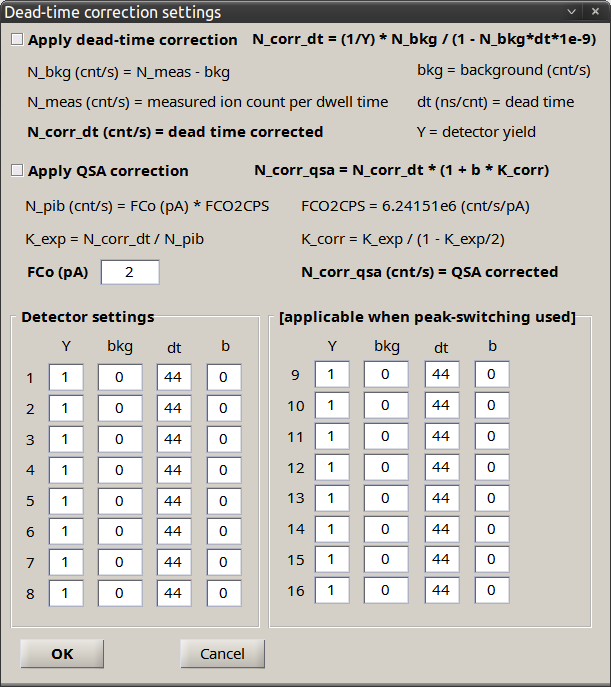
\includegraphics[scale=0.4]{figs1/LANS-dt-qsa-settings}
\caption{\label{fig:dtqsa}%
LANS window where you can adjust settings for dead-time and QSA corrections.}
\end{figure}

\s{Select \lans{Input} $\ra$ \lans{Ask for range of planes and masses before loading} if you want to interactively define \bb{a range} of planes and masses that should be extracted during loading of the raw dataset.}

\nnb{This is unnecessary in most cases, but it may be required if your dataset is huge (e.g., more than 1~GB of data) and the memory (RAM) on your computer is insufficient.}

\s{Select \lans{Input} $\ra$ \lans{Shift columns or rows when loading raw data}.}

\nb{This data correction is relevant for data acquired by the NanoSIMS 50L instrument at Utrecht University and probably very few others around the world. It concerns a glitch in the acquisition software, which causes the data in pixels from the first column (or row) to appear in the last column (or row), or vice versa. This option allows you to \bb{shift} the pixels to the \bb{correct} position during loading of the raw dataset by entering 1 and 0 in the corresponding fields (Fig.~\ref{fig:shiftrowcolumn}). You can skip this step if this is not an issue in your dataset.}

\begin{figure}[!ht]
\centering
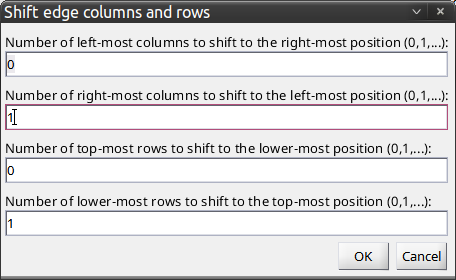
\includegraphics[scale=0.5]{figs1/LANS-shift-rows-columns}
\caption{\label{fig:shiftrowcolumn}%
LANS window where you can adjust how rows and columns in the input raw image data should be shifted during loading.}
\end{figure}

\s{Select \lans{Input} $\ra$ \lans{Load RAW dataset} to load the raw dataset from disk in a standard way (i.e., plane by plane). When searching for the dataset, choose the file type: \ttt{im.zip} or \ttt{im}, depending on whether the raw data has been compressed or not. After selecting the raw data file, observe the progress of loading in the Matlab console.}

\nb{When the loading is finished, names of the masses will automatically be filled in the corresponding \lanstf{mass} text fields. Additionally, \ttt{[]} will be added in the \lanstf{planes} text field, which stands for ``all planes''.}

\nb{Sometimes, the mass name entry in the binary \ttt{im} file is incorrectly saved. If this happens, a~``strange-looking'' name such as \ttt{au32} will be filled as the corresponding \lanstf{mass}, referring to the actual mass detected (in atomic units). If you know that the detected isotope was (in this example) ${}^{32}$S, you can rewrite the string from \ttt{au32} to \ttt{32S} and use it as the name of the mass in further analysis.}

%%

\subsection{Display of mass images plane-by-plane}
\setcounter{step}{0}
\label{sec:display-masses-plane-by-plane}

\vskip2.5mm

\s{Select \lans{Input} $\ra$ \lans{Autoscale plane images} to automatically fill in the \lanstf{scale} for each detected mass.}

\nnb{The scale, in the form of \ttt{[min max]}, is calculated as the 0.001 and 0.999 quantile of the ion counts across all pixels and planes. The quantiles can be adjusted using \lans{Preferences} $\ra$ \lans{Additional output options} (see auto-scaling in Section~\ref{sec:appearance1}). }

\s{In the \ttt{Detected masses} box, check the \lanscb{checkboxes}  to the left from the \lanstf{masses} to select which masses will be displayed in the following step.}

\nnb{By default, all masses are selected, but you may want to change it.}

\s{Select \lans{Input} $\ra$ \lans{Display plane images for all masses} to view secondary ion counts detected in individual planes for \bb{all} masses (Fig.~\ref{fig:displayplanes}).}

\purplebox{}
This shows the actual data in its \bb{rawest} form, i.e., \bb{ion counts per pixel per plane.}
\tcbe

\begin{figure}[!ht]
\centering
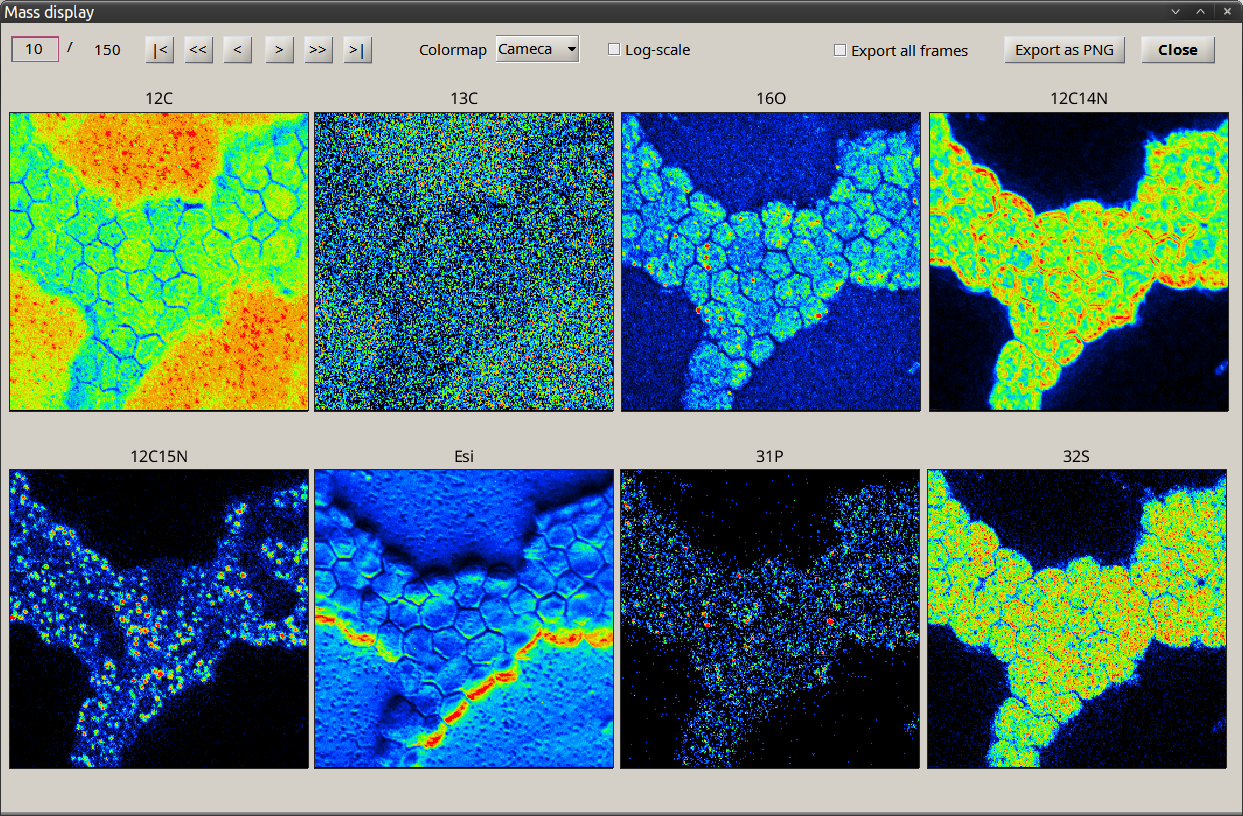
\includegraphics[width=\textwidth]{figs3/LANS-display-planes-raw}
\caption{\label{fig:displayplanes}%
LANS window for viewing the raw image data for all detected masses, plane by plane.}
\end{figure}

\sbx{Use arrows to browse through the planes forward and backward.}

\s{Click on \lans{Export as PNG} if you want to export all masses in a particular plane as a PNG file. If you additionally check \lanscb{Export all}, you can export all planes, each into a separate PNG file.}

\s{When browsing through the ion count images, you can often notice a small \bb{drift} when going from one plane to the next. This drift is caused by temperature instabilities during the measurements (a~bigger jump can also be caused by an~earthquake!). You will be able to correct for this drift in the next step. At this point, you should \bb{decide} on the mass that will be used to calculate the drift correction (called \lanstf{Base mass for alignment}).}

\nb{As a~rule of thumb, it should be one with a relatively \bb{high ion counts} and \bb{clear contrast} across the image. In this example, it will be \ttt{12C14N}. For many datasets, \ttt{Esi} is also a~good candidate.}

%%

\newpage

\subsection{Drift-correction and accumulation of planes}
\setcounter{step}{0}
\label{sec:drift-correction-accumulation}

\goldbox{}
The drift-corrected accumulation of planes is controlled by settings specified in the \ttt{Accumulation options} box and by the numbers in the \lanstf{planes} list (Fig.~\ref{fig:alignoptions}). 
\tcbe

\begin{figure}[!ht]
\centering
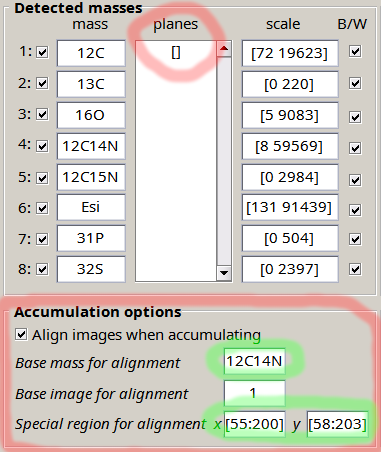
\includegraphics[scale=0.4]{figs3/LANS-main-alignment}
\caption{\label{fig:alignoptions}%
Parts of the main LANS window relevant for controling drift-correction of planes.}
\end{figure}

\s{Specify the \lanstf{Base mass for alignment}. This is done based on your choice made in the previous step (in this example: \ttt{12C14N}).}

\s{Select \lans{Input} $\ra$ \lans{Display alignment mass}. }

\s{In the new window that opens (Fig.~\ref{fig:show-alignment-mass}), click on \lans{arrows} to browse through the individual planes. }

\begin{figure}[!ht]
\centering
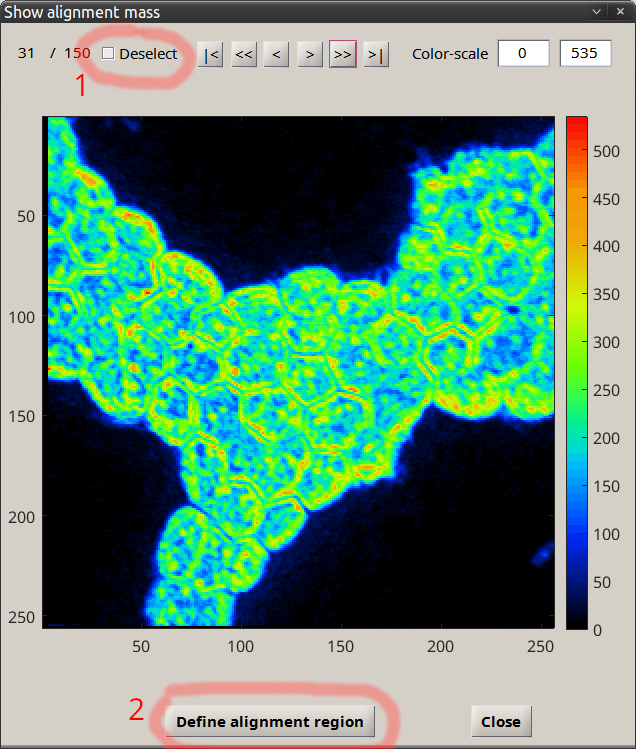
\includegraphics[scale=0.4]{figs3/LANS-show-alignment-mass}
\caption{\label{fig:show-alignment-mass}%
LANS window where you can (1) specify planes that should be excluded during accumulation and (2) define a~region based on which drift-correction will be calculated.}
\end{figure}

\s{Check \lanscb{Deselect} to mark the plane that should be excluded from accumulation (e.g., if the data in that plane is corrupt).}

\s{After you have completed the plane selection, click on the \lans{Define alignment region} button to define an area in the image based on which the drift correction will be calculated in the next step.}

\nb{It is recommended to define this area as a~minimum rectangular region in the image that contains pronounced spatial heterogeneities (such as a cell or a group of cells).}

\s{Close the window when you have defined the area.}

\nb{After you close the window, the x and y ranges of the alignment region will be written in the respective fields of \lanstf{Special region for alignment} in the main LANS window (Fig.~\ref{fig:alignoptions}). Also, the range of selected planes will be written in the \lanstf{planes} list. You can edit these fields if you know the correct values, but be careful not to make any syntax errors. }

\s{Back in the main LANS window, check \lanscb{Align images when accumulating} if you want to apply automated drift correction during the accumulation of planes. If not, which is rarely the case, leave this checkbox unchecked.}

\s{Select \lans{Input} $\ra$ \lans{Accumulate plane images} to start the accumulation of drift-corrected images. }

\nb{You will be asked whether to employ a \lans{New} or \lans{Old} algorithm. In most cases, you will choose the \lans{New} one. However, the old one is preferred if the drift-correction is based on images with very low ion counts (i.e., very pixelated images).}

\sbx{Observe the drift-correction progress in the Matlab console. }

\s{When the drift-correction information is calculated for all selected planes, you will be prompted to accept or reject it (Fig.~\ref{fig:drift-correction}). }

\begin{figure}[!ht]
\centering
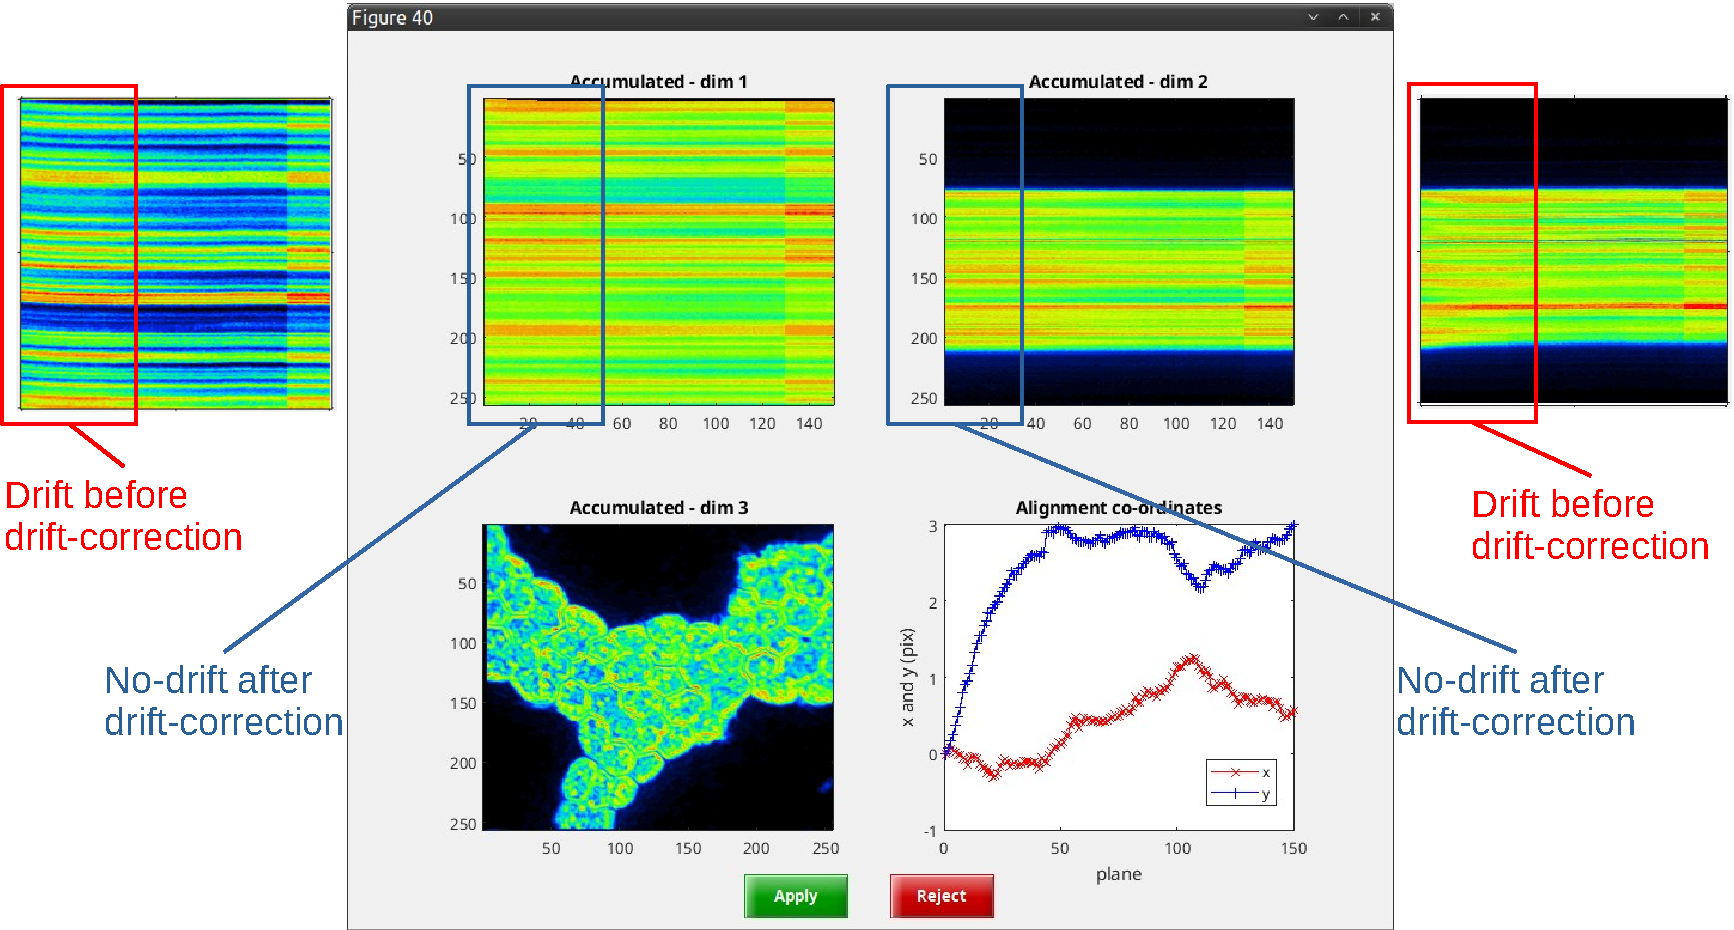
\includegraphics[width=\textwidth]{figs3/LANS-drift-correction}
\caption{\label{fig:drift-correction}%
LANS window showing the results after calculating the drift-correction (central window). For comparison, the original ion count data along a~vertical and horizontal profile through the center of the image are also shown (to the left and right of the central window). In this example, the drift along the vertical ($y$) direction was pronounced during the initial 50 planes (by about 3~pixels), then decreased. The drift in the horizontal ($x$) direction did not exceeed about 1.5 pixels across the 150 planes. The drift-correction is considered good if the two images in the top row (`Accumulated dim 1 and 2') show \bb{flat horizontal stripes}, in contrast to `wiggly' stripes visible in the data before drift correction.}
\end{figure}

\nnb{If you \lans{accept} it, the information will be stored in the file \ttt{xyalign.mat} and all planes for all masses will be accumulated based on this information. Also, this information will automatically be used in the future if you load the raw dataset using \lans{Input} $\ra$ \lans{Load+accumulate+display RAW} \lans{or PROCESSED dataset}.}

\nnb{If you \lans{reject} it, you can reiterate the previous steps (1--4) until you arrive at a dataset with drift-corrected and accumulated planes.}

\nb{Note that you \bb{do} need to accumulate the planes, because most of the subsequent data processing steps only work for the ion counts accumulated over all (selected) planes.}

\nb{If you realize, anytime at a later point during your data processing, that you are not satisfied with the drift-correction, you need to first delete the \ttt{xyalign.mat} file (via \lans{Preferences} $\ra$ \lans{Remove xyalign.mat from disk}), then \lans{Load RAW dataset}, and then repeat the previous steps (S1--S10) to drift-correct and accumulate the planes again.}

%%

\subsection{Display accumulated mass images}
\setcounter{step}{0}

\vskip2.5mm

\s{Back in the main LANS window, select \lans{Input} $\ra$ \lans{Autoscale accumulated images} to update the \lanstf{scale} fields with a range optimized for displaying accumulated mass images. }

\nb{The optimum scale is calculated as the 0.001 and 0.999 quantiles of the accumulated ion counts across the image pixels. These quantiles can be adjusted via \lans{Preferences} $\ra$ \lans{Additional output options}.}

\s{Alternatively, define the \lanstf{scale} \bb{manually} by typing in the \ttt{[min max]} (minumum and maximum) values by yourself. If you then press \ttt{Enter}, the corresponding mass will be displayed in a new window using the color scale defined by the specified range. You can repeat this many times to \bb{quickly adjust} the color scale for optimal display (e.g., to achieve best contrast).}

\nb{Note that you can display the images in multiple colormaps. These can be adjusted via \lans{Preferences} $\ra$ \lans{Additional output options} (see Section~\ref{sec:appearance1}). Explore them to find the best you like. If you want to display the images in grayscale, click on the corresponding \lanscb{B/W} checkbox next to the scale.}

\nb{If there is a large contrast in ion counts across the image (e.g., by 2--3 orders of magnitude), it is often useful to display the log-transformed image. To do this, check \lanscb{Log10-transform} in the \ttt{Output options} box before you press \ttt{Enter} to display the image. When displaying log-transformed images, make sure that the minimum value of the \lanstf{scale} is greater than 0. If it is 0 and you press \ttt{Enter}, the image will be displayed in a~scale where $\ttt{min} = 0.001\times\ttt{max}$, which may not be optimal.}

\s{Select \lans{Input} $\ra$ \lans{Display accumulated images for all masses} to display the images, lumped together for all masses, and export them in a PNG file (Fig.~\ref{fig:display-accu-planes}). This output is useful as a~quick overview of the accumulated raw data.}

\begin{figure}[!ht]
\centering
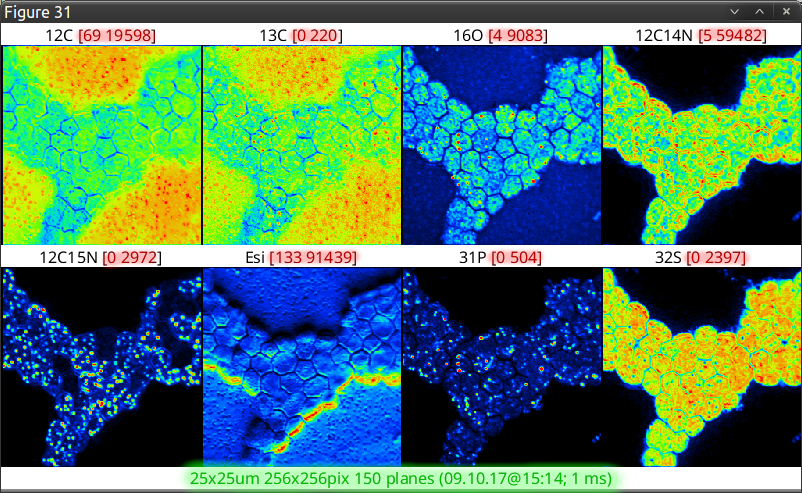
\includegraphics[width=\textwidth]{figs3/LANS-display-accu-planes}
\caption{\label{fig:display-accu-planes}%
Display of ion counts after drift-correction and accumulation of selected planes. The scale is shown for each individual mass, formatted as \ttt{[min max]}. Basic information about the data, e.g., real and pixel size, date of acquisition, dwell time, is also shown (at the bottom).}
\end{figure}

\s{Check \lanscb{Display images} in the \ttt{Output options} box and then select \lans{Output} $\ra$ \lans{Display masses} to display the images in a~nicer way and separately for each mass (Fig.~\ref{fig:display-masses}). }

\begin{figure}[!ht]
\centering
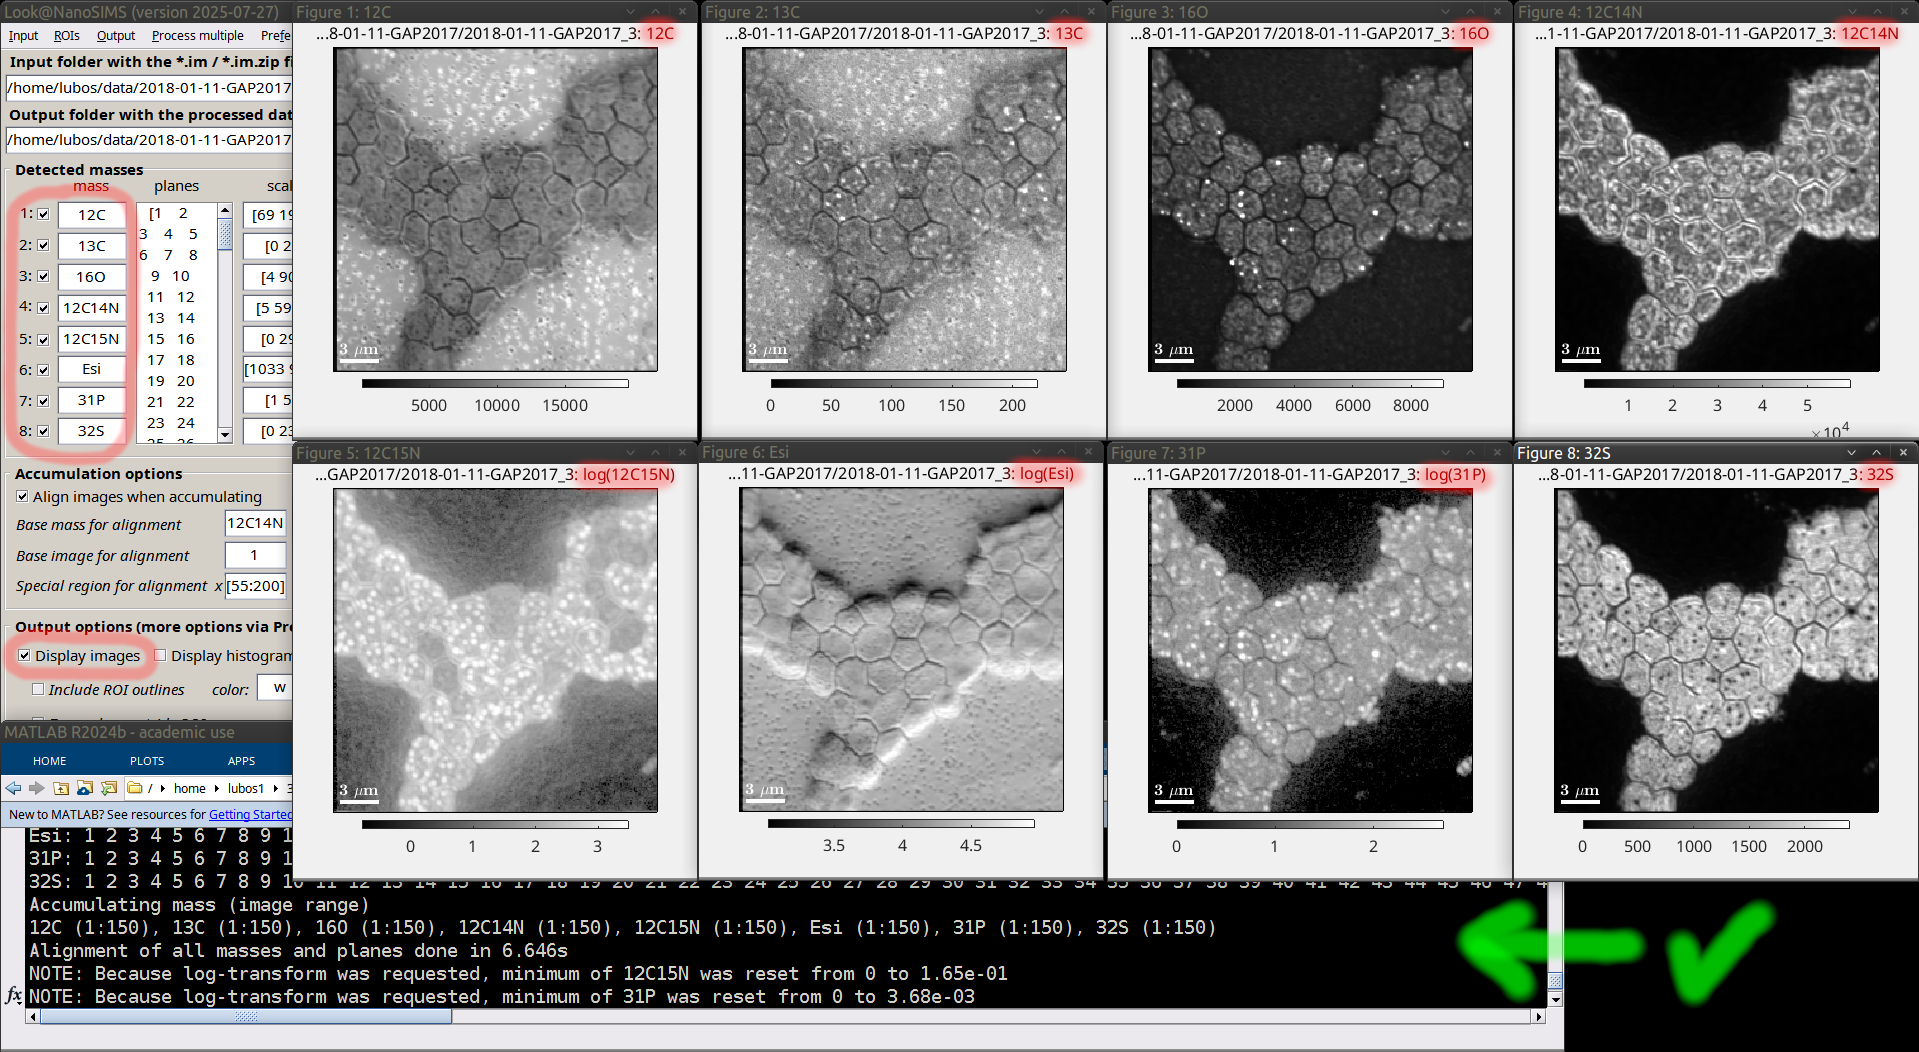
\includegraphics[width=\textwidth]{figs3/LANS-display-masses}
\caption{\label{fig:display-masses}%
Screenshot of a~LANS session showing ion count images after drift-correction and accumulation. Each mass is displayed in a~separate window, some in the linear scale, some in the logarithmic scale. Note the \bb{arrangement} of the main LANS window in the top-left part of the screen and of the Matlab console at the bottom of the screen, which allows monitoring of messages reported by LANS at all times.}
\end{figure}

\nb{In this step, the image appearance, including the location of the colorbar, size and location of the scale bar, etc., can be tweaked via \lans{Preferences} $\ra$ \lans{Additional output options} (see Section~\ref{sec:appearance}). }

\purplebox{Remember}
When displaying the images, ensure that \lanscb{Export PDF graphics} in the \ttt{Output options} box is checked. This will allow you to \bb{export} the images in a~PDF format (they will be stored in the \ttt{pdf} sub-folder of the current data folder). If this checkbox is not checked, no output will be generated, and you may be left wondering: why doesn't it work?!
\tcbe

%%

\subsection{Display ratio images}
\setcounter{step}{0}

\vskip2.5mm

\s{Back in the main LANS window, type \bb{formulas} for calculating ratio images in the  \lanstf{expression} fields (Fig.~\ref{fig:display-ratios}). In principle, the formula can be any valid arithmetic expression containing any of the detected masses. However, it is recommended not to make the formulas too complicated. Typical examples include:

\begin{itemize}
\item \ttt{13C/12C} to calculate the $^{13}C/^{12}C$ isotope ratio,
\item \ttt{13C/(12C+13C)} to calculate the $^{13}C$ atom fraction,
\item \ttt{32S/12C} to calculate the $^{32}S/^{12}C$ ion count ratio (a proxy for the S/C elemental ratio), 
\item \ttt{31P/plane} to calculate the average $^{31}P$ ion counts per detected plane, 
\item \ttt{31P/plane/pixel} to calculate the average $^{31}P$ ion counts per plane per pixel (only applicable if ROIs are defined; see below).
\end{itemize}}

\s{For each expression, type in the \lanstf{scale} to the correspoding field (Fig.~\ref{fig:display-ratios}). Similar to masses, the scale should be in the form \ttt{[min max]} (minumum and maximum). }

\nb{If you then press \ttt{Enter}, the corresponding ratio image will be displayed in a~new window using the color scale defined by the specified range. You can repeat this many times to \bb{quickly adjust} the color scale for optimal display.}

\s{Check \lanscb{Display images} in the \ttt{Output options} box and then select \lans{Output} $\ra$ \lans{Display ratios} to display the ratio images, in in a~separate window (Fig.~\ref{fig:display-ratios}). }

\begin{figure}[!ht]
\centering
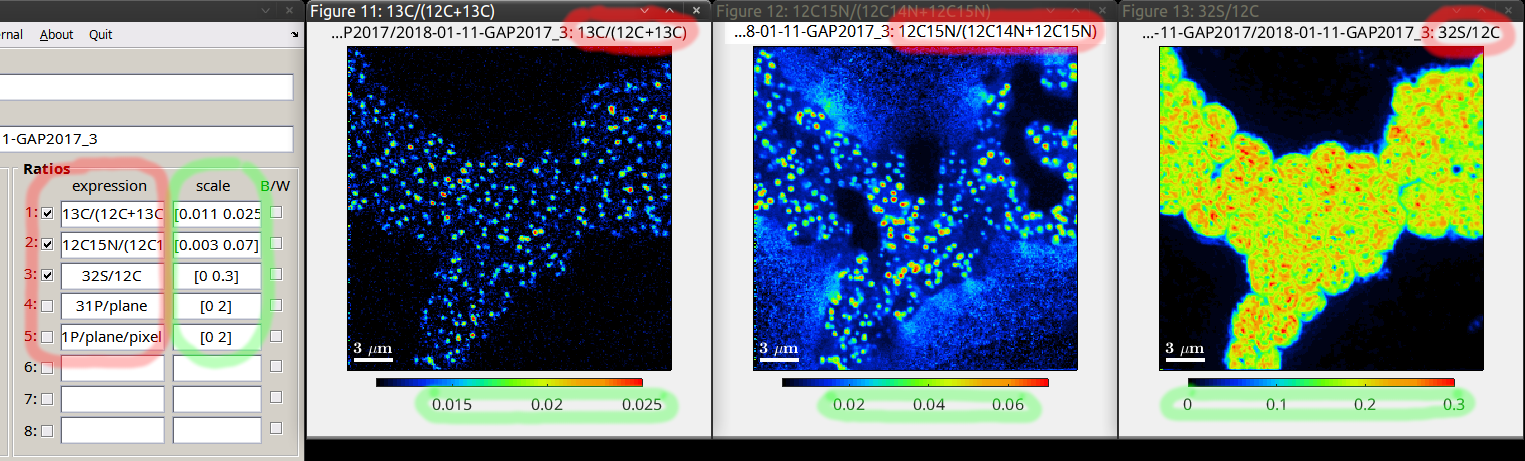
\includegraphics[width=\textwidth]{figs3/LANS-display-ratios}
\caption{\label{fig:display-ratios}%
Examples of ion count ratio images. The ratios are defined through formulas typed in the \lanstf{expression} field (marked in red), the scales are defined in the corresponding \lanstf{scale} fields (marked in green).}
\end{figure}

\nb{In this step, the image appearance can be tweaked via \lans{Preferences} $\ra$ \lans{Additional output options}.}

\nb{As emphasized above, ensure that \lanscb{Export PDF graphics} in the \ttt{Output options} box is checked to export the images as PDF.}

%%

\subsection{Display RGB overlays}
\setcounter{step}{0}

\goldbox{}
To increase the information value of the mass and ratio images, they can be combined and displayed as RGB overlays.
\tcbe

\s{To specify which image will be filled in the red, green and blue channel of the RGB overlay, enter identification numbers (1--8, found to the left of the mass names or ratio expressions) in the corresponding \lanstf{R/x}, \lanstf{G/y} and \lanstf{B/z} fields (found under \ttt{Plot-x-y-z graph} in the \ttt{Output options} box) (Fig.~\ref{fig:rgb-overlay}).}

\begin{figure}[!ht]
\centering
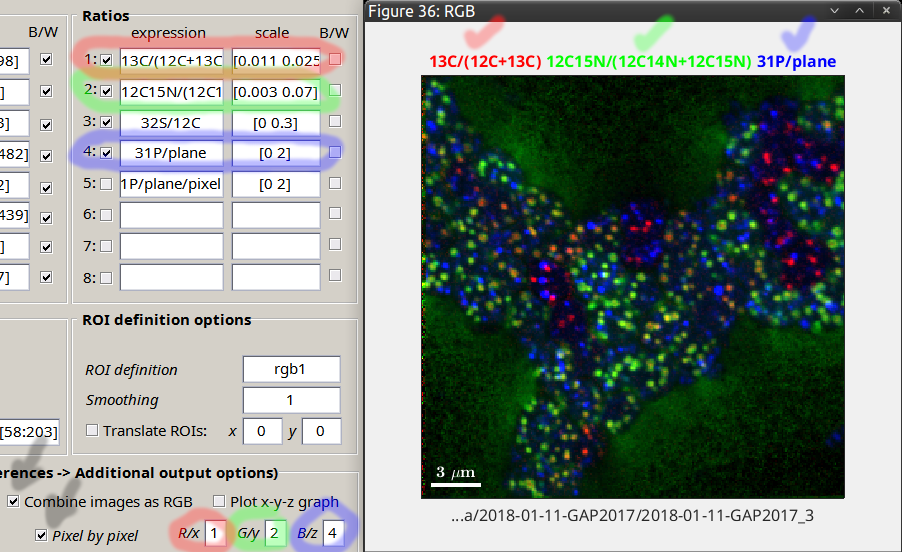
\includegraphics[scale=0.35]{figs3/LANS-rgb-overlay}
\caption{\label{fig:rgb-overlay}%
Example of an RGB overlay of ion count and ion count ratio images.}
\end{figure}

\nbx{At most one number per R, G and B field is allowed. If one or more of the fields is left empty, the corresponding channel(s) will be set to zero and thus appear black in the RGB overlay.}

\s{In the \ttt{Output options} box, check \lanscb{Combine images as RGB}. Then, check \lanscb{Pixel by pixel} to combine the images without modification and/or \lanscb{ROI-averaged} to use ROI-averaged values when creating the overlays (the latter is only possible if ROIs have been defined).}

\s{Select \lans{Output} $\ra$ \lans{Display masses} or \lans{Display ratios} to display the RGB overlay derived from mass or ratio images, respectively.}

\nb{If you want to overlay a~mass image with a~ratio image, enter the corresponding name of the mass into one of the \lanstf{expression} fields, specify the scale, enter the corresponding identification number in one of the \lanstf{color} fields (R, G or B), and then select \lans{Output} $\ra$ \lans{Display ratios} (Fig.~\ref{fig:rgb-overlay}). }

\nnb{You can combine multiple masses with multiple ratios by entering the corresponding identification numbers in the R, G and B fields.}

\nnb{In addition to PDF, RGB overlay images are also exported as TIF files (in the \ttt{tif} sub-folder of the dataset folder).}

%%

\subsection{Define ROIs}
\setcounter{step}{0}

\goldbox{}
Typically, much of nanoSIMS data analysis revolves around regions of interest (ROIs). There are many options for defining ROIs in LANS, as described below. Once you get used to it and learn the ``tricks'', ROI definition in LANS can be very efficient. 
\tcbe

\purplebox{Remember}
Here, we re-emphasize the importance of looking at the instructions and comments written in the Matlab console while defining ROIs. They provide more details about what \bb{exactly} you need to do while performing specific steps, and how to finish them correctly. The key rule is: \textcolor{red}{\bb{if you start an action, you \emph{must} complete it.}} More specifically, if you start one particular action (e.g., ROI definition by manual drawing) and then select a~different action from the menu or using a~keyboard short-cut (e.g., removing a~ROI or zooming in the image) \bb{before} completing the previous action, the program will likely get ``stuck'' or perform illogical actions. This may lead to loosing the currently or previously defined ROIs, or even the need to terminate the ROI definition tool. Moreover, it may give you a~wrong impression that LANS is not a~good tool. We hope that you will not get that far, because LANS \bb{is} a~very efficient tool! However, you do need to give yourself enough time to learn the tricks and ultimately memorize the exact sequence of mouse-clicks and keyboard presses you need to make, as instructed in the console, in order to get the work done. It is a~very good idea that you practice the ROI definition steps for some time before you continue with a~more serious work!  We won't go into details here, but briefly, this peculiarity of LANS is related to the way Matlab handles user's mouse and keyboard inputs in a~mode that allows drawing of objects within a~figure. You can learn more about this topic via \lans{Help} provided in the ROI definition tool window.
\tcbe

\s{In the main LANS window, specify the \lanstf{ROI definition template}. }

\nnb{This can be an individual mass, ratio, an RGB overlay of masses or ratios, or an external image.}

\nnb{In this example, we will use an RGB overlay of \ttt{12C15N/(12C14N+12C15N)}, \ttt{12C14N} and \ttt{31P} (Fig.~\ref{fig:roi-template}). Since we want to combine ratios and masses, we enter \ttt{12C14N} as, e.g., expression~6, \ttt{31P} as expression~4, and enter the scale for both in the corresponding \lanstf{scale} field. Then, we enter \ttt{2}, \ttt{6} and \ttt{4} to the fields for \lanstf{R}, \lanstf{G} and \lanstf{B}, respectively. Finally, we enter \ttt{rgb2} as the \lanstf{ROI definition template} (entering \ttt{rgb} means that we use an RGB overlay, \ttt{2} means that we use an overlay of ratios rather than masses).}

\begin{figure}[!ht]
\centering
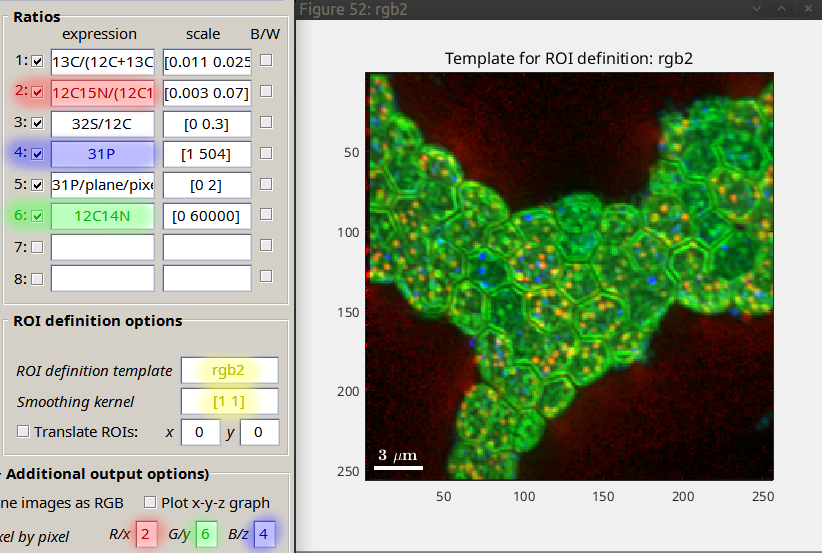
\includegraphics[scale=0.4]{figs3/LANS-roi-template}
\caption{\label{fig:roi-template}%
Example showing how to define a~ROI definition template. In this example, the template comprises an RGB overlay of three ratio images (\ttt{rgb2}).}
\end{figure}

\nnb{The ROI template can optionally be \bb{smoothed} before it is used for ROI definition. Smoothing is done using a median filter with a~two-dimensional kernel size (in pixels) specified in the \lanstf{Smoothing kernel} field. If applied, ROI outlines will generally be smoother if defined using the \lans{interactive thresholding} approach (see below). In this example, we will not do any smoothing and just use \ttt{[1 1]} as the smoothing kernel (Fig.~\ref{fig:roi-template}).}

\s{Select \lans{ROIs} $\ra$ \lans{Display template for ROI definition} to verify that the template looks as intended (Fig.~\ref{fig:roi-template}). }

\s{Select \lans{ROIs} $\ra$ \lans{INTERACTIVE ROIs definition tool} to open a~window dedicated to ROI definition. }

\nb{During this process, you will be prompted to select the \ttt{ROI file} (e.g., \ttt{ROIs.mat}) and \ttt{ROI classification file} (e.g., \ttt{ROIs.dat}). Select them if the files have been previously created and you want to reuse them, or press \lans{Cancel} if they do not exist (yet).}

\nb{If they exist and you do select them both, they will be \bb{linked}. This means that when you add or remove a~ROI from the image file, the corresponding ROI will also be added or removed from the classification file. This will be explained in more details later on.}

\goldbox{}
After these steps, a new window will open (Fig.~\ref{fig:roi-definition-tool}), allowing you to define, display and save ROIs, as explained in the following.
\tcbe

\begin{figure}[!ht]
\centering
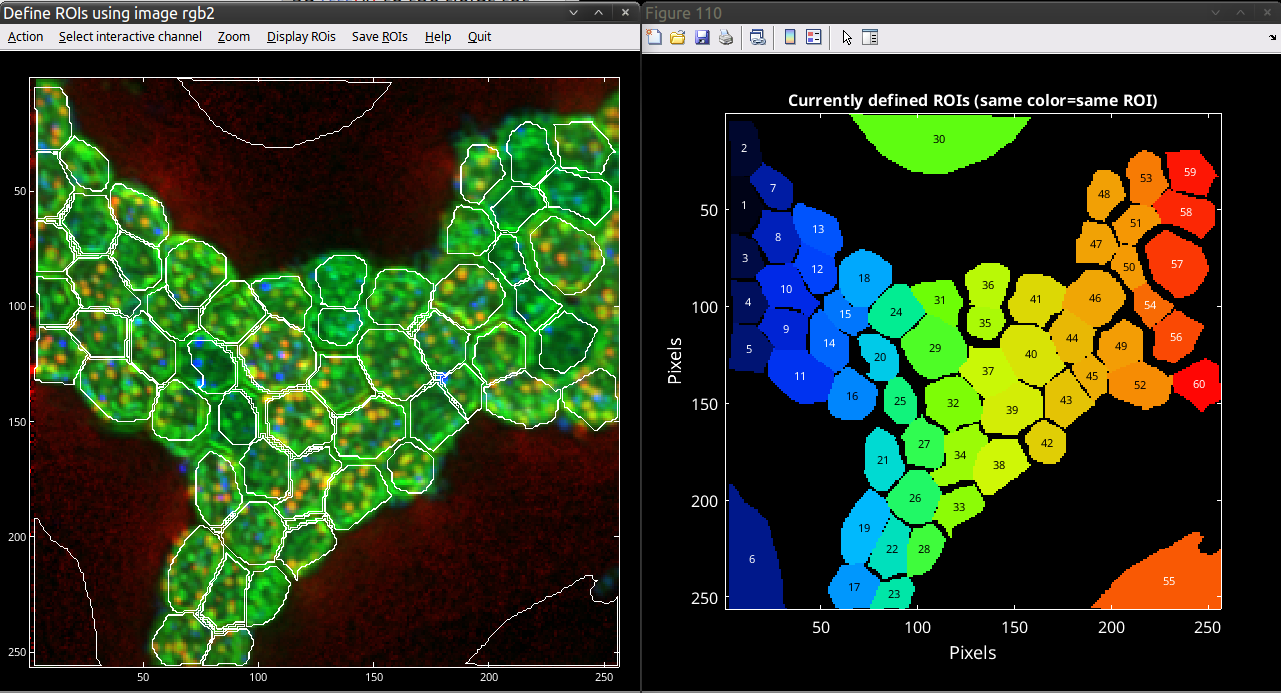
\includegraphics[width=\textwidth]{figs3/LANS-roi-definition-tool}
\caption{\label{fig:roi-definition-tool}%
Definition of regions of interest (ROIs) in LANS. The left window provides tools for manual or semi-automated definition of ROIs, the right window shows the currently defined ROIs. The defined ROIs are displayed as outlines in the left window and colored areas in the right window. Note that the ROIs are numbered such that the ROI's central points increase from left to right. Also note the Help in the menu, where you can learn more details and useful tricks.}
\end{figure}

\setcounter{step}{0}

\s{In the ROI definition window, select \lans{Action} $\ra$ \lans{Draw ROIs freehand} (\ttt{Ctrl+d}) to draw a ROI using a mouse.}

\purplebox{Example of instructions you need to follow, step-by-step}

\begin{itemize}
\item Click the left mouse button, hold it, and \bb{draw} a~region of interest. 
\item After releasing the mouse button, the initial and final points defined by the mouse will be connected.
\item At this point, you will be still able move the ROI around using a mouse.
\item Double-click on the ROI to \bb{confirm} its final position.
\item When prompted, specify whether the ROI outline should be defined as the \lans{coarse polygon} you have just drawn or as an \lans{ellipse that circumscribes} this polygon. Typically, you will choose the first option: coarse polygon. 
\item At this point, you can also \bb{cancel} the ROI definition by selecting \lans{Do not take anything} or pressing the \ttt{ESC} key.
\item You \bb{must} finish ROI definition by either confirming or canceling it.
\end{itemize}
\tcbe

\s{Experiment with different ways of defining ROIs, such as drawing them as \lans{ellipses} (\ttt{Ctrl+e}) or \lans{rectangles} (\ttt{Ctrl+t}), or via \lans{Interactive thresholding}. In certain situations, the last approach is particularly useful and will be described in greater detail later on.}

\nb{Practice ROI definition and remember: after drawing a~ROI, you always need to double-click on it to confirm its size and location.}

\nb{If you draw a ROI over another, previously defined ROI, the last one will take the priority. In this way, you can draw a~ROI inside a~ROI (but not a~ROI outside a~ROI).}

\nb{If you click within the ROI outline, the ROI identifier (number) will be displayed in the Matlab console.}

\nb{ROIs are renumbered everytime you add or remove a~ROI, such that the ROIs' central points increase from left to right.}

\s{Select \lans{Display ROIs} $\ra$ \lans{Display ROIs with ROI ID's} (\ttt{Ctrl+w}) to display the currently defined ROIs.}

\nb{By default, they will be displayed in a~window placed \bb{just to the right} from the window of the ROIs definition tool (Fig.~\ref{fig:roi-definition-tool}). Thus, it is recommended that you keep the latter window somewhere on the left side of your screen. If you had placed that window near the right edge of your screen, it might happen that the window with the ROIs would be invisible (because it would be placed to the right of the tool window, i.e., outside of your screen).}

\nnb{Notice that ROI identification numbers (IDs) are generated automatically and increase from left to right when sorting the ROIs based on their central point.}

\nb{If you want to display ROIs with specific IDs, you can do so by typing the IDs in the dialog that opens after you choose to display the ROIs.}

\nb{If the ROIs have been classified, you can display ROIs from a~specific class by typing the corresponding class identification letter, rather than the ROI identification number, in the same dialog.}

\s{Explore the \lans{Action} menu to test various ways to \lans{define}, \lans{split}, \lans{merge}, or \lans{remove} ROIs.}

\s{Use the \lans{Zoom} menu to zoom in the ROI definition image or zoom out.}

\nb{This brings about another Matlab-related peculiarity: Once you select \lans{Zoom} $\ra$ \lans{Zoom ENABLE} (\ttt{Ctrl+z}), you \bb{enter} a~`zoom' mode. In this mode, you can use the mouse to specify the zoomed-in area. Subsequently, you must \bb{quit} the `zoom' mode by selecting \lans{Zoom} $\ra$ \lans{Zoom DISABLE} (or pressing \ttt{Ctrl+z} again). Only then can you proceed with other actions.}

\s{Select \lans{Save ROIs} from the menu, or press \ttt{Ctrl+s}, to save the currently defined ROIs. }

\nb{You can choose the default name (e.g., \ttt{ROIs.mat}) or a different name (e.g., \ttt{cells.mat}).}

\purplebox{No undo!}
Note that there is \bb{no undo} function implemented in LANS (yet). Thus, it is recommended that you save the ROIs frequently, or at least after you have made an effort to define a~few complicated ROIs that you do not want to loose.
\tcbe

\s{When you are satisfied with the defined ROIs and are almost certain that you defined all of them, select \lans{Display ROIs} $\ra$ \lans{Display ROIs with ROI ID's} (\ttt{Ctrl+w}) to display them all again. This will set the floor for the next step: ROI classification.}

%%

\subsubsection{ROI definition via interactive thresholding}
\setcounter{step}{0}

\goldbox{}
Before continuing with ROI classification, we describe an example of how to define ROIs via interactive thresholding. In general, once you get used to it and learn the tricks, this approach allows you to define ROIs more efficiently and reproducibly than by drawing them manually. However, the approach is only applicable if the signal used for recognizing the ROI \bb{stands out} relative to the surrounding background.
\tcbe

In this particular example, you will draw a~ROI that corresponds to a~cyanophycin inclusion inside one of the cells. The inclusion is characterized by a~pronounced enrichment in the ${}^{15}N$ isotope relative to the cell biomass. Because the ${}^{15}N$ atom fraction (i.e., the ratio \ttt{12C15N/(12C14N+12C15N)}) is used as the red channel in the ROI definition template, the inclusion can be recognized as an~orange spot (it contains $CN$ in green, and high ${}^{15}N$ in red).

\s{In the ROI definition tool window, zoom in to a group of cells with clear orange spots (e.g., as shown in Fig.~\ref{fig:roi-interactive5}A).}

\s{Because an RGB overlay is now used as a~ROI definition template, the interactive channel needs to be defined first. As mentioned above, the red channel will be the interactive one in this example. Hence, choose \lans{Select interactive channel} $\ra$ \lans{Red} from the menu. }

\nnb{This step would not be necessary if only one channel was used as the ROI definition template. }

\nb{Note that through the \lans{Select interactive channel} menu, you can also choose which of the RGB channels should be displayed or hidden during ROI definition (compare panels A--D and E in Fig.~\ref{fig:roi-interactive5}). You can do this also more quickly by pressing \ttt{Ctrl+1}, \ttt{Ctrl+2} or \ttt{Ctrl+3} to hide or show the R, G or B channel, respectively.}

\begin{figure}[!b]
\centering
\begin{tabular}{cccccc}
A: \includegraphics[scale=0.23]{figs3/LANS-roi-interactive0}
&
B: \includegraphics[scale=0.23]{figs3/LANS-roi-interactive1}
&
C: \includegraphics[scale=0.23]{figs3/LANS-roi-interactive2}
\\[5mm]
D: \includegraphics[scale=0.23]{figs3/LANS-roi-interactive3}
&
E: \includegraphics[scale=0.23]{figs3/LANS-roi-interactive4}
&
F: \includegraphics[scale=0.23]{figs3/LANS-roi-interactive5}
\end{tabular}
\caption{\label{fig:roi-interactive5}%
ROI definition via the interactive thresholding approach. (A)~A~zoomed-in area in the image, with no ROI yet defined. (B)~A~ROI outline (in white) is drawn automatically by selecting the red channel as the active one, starting the interactive thresholding mode, and clicking on the pixel indicated. The selected area can be enlarged~(C) or made smaller~(D) by repetatively pressing the \ttt{up} or \ttt{down} arrow keys while the interactive thresholding mode is active. The ROI is confirmed by pressing \ttt{Enter}, which will stop the interactive thresholding mode. (E)~Image of the same area but with the green channel hidden from view. (F)~If the green channel, instead of the red one, was selected as the active one, interactive thresholding would draw ROI based on the intensity of the green colour. In this particular case, this approach would not be very useful for defining ROIs corresponding to individual cells, because the cells are not well separated from each other (although they do stand out relative to the background filter). This may be different in other datasets, however, allowing rapid definition of ROIs corresponding to cells.}
\end{figure}

\s{Select \lans{Action} $\ra$ \lans{Interactive thresholding} (\ttt{Ctrl+a}) to start ROI definition via interactive thresholding.}

\s{Click with a~left-mouse button on the image in a~pixel with a~high signal of the active channel (i.e., somewhere on the orange spot).}

\nb{You will notice that a~ROI outline is automatically drawn (Fig.~\ref{fig:roi-interactive5}B). The outline corresponds to a~contour where the signal values (of the active channel) do not fall below the value in the selected (clicked) pixel multiplied by a~\bb{threshold} value.}

\s{The threshold value is 0.5 by default, but it can be changed interactively by pressing (\bb{slowly}) the \lans{up} or \lans{down} arrow key.}

\nb{When doing so, the ROI outline will cover a~larger (Fig.~\ref{fig:roi-interactive5}C) or smaller (Fig.~\ref{fig:roi-interactive5}D) area, respectively. Keep pressing the \lans{up} or \lans{down} arrow key, repetitively but \bb{slowly}, to observe this behaviour. This is the \bb{essence} of the interactive thresholding approach!}

\nnb{If a~different pixel is selected (clicked), the ROI outline is automatically redrawn according to value in the clicked pixel and the current threshold.}

\purplebox{Note on optimization}
By combining left-button mouse clicks with the \lans{up} and \lans{down} arrows, you can rapidly optimize the ROI definition using the \lans{Interactive thresholding} approach.
\tcbe

\s{When you are satisfied with the defined ROI (e.g., if the defined ROI looks as shown in Fig.~\ref{fig:roi-interactive5}D), \bb{press \ttt{Enter} to confirm it}. Alternatively, press \bb{\ttt{Esc}} if you want to cancel the current interactive ROI definition.}

\purplebox{Reminder}
This is another possible moment when you can get ``stuck'' if you do not correctly follow the sequence of steps described above. Thus, we repeat the key rule: \bb{if you start} the \lans{Interactive ROI definition} sequence of actions, \bb{you \emph{must} terminate it} properly by pressing either \ttt{Enter} (to confirm the ROI) or \ttt{Esc} (to cancel the interactive ROI definition). You must \bb{not} start any other action (such as new type of ROI definition, ROI removal, zooming in, display of ROIs, etc.) before finishing the previous one with \ttt{Enter} or \ttt{Esc}.
\tcbe

\s{At this point, it is recommended that you spend some time practicing the above sequence of steps. Once you get used to it, it can fairly substantially speed up your ROI definition.}

\s{Note that the interactive thresholding approach is, essentially, an automatic drawing of a~contour at a~particular height on a~\bb{hill}. If you want to apply the same approach but for a~\bb{valley}, you need to convert valleys into hills and vice versa. You can do this by selecting \lans{Action} $\ra$ \lans{Invert template image} (Fig.~\ref{fig:interactive-invert}). When doing so, it will probably be a~good idea to also change the color of the ROI contour line (e.g., from the default \ttt{w}hite to blac\ttt{k}), which you can do by selecting \lans{Action} $\ra$ \lans{Change color of the ROI outline}. Then continue in the same way as described above (steps S3--S6) to define a~ROI. You can always get back to the original template by inverting it again.}

\begin{figure}[!ht]
\centering
\begin{tabular}{ccc}
A: \includegraphics[scale=0.19]{figs3/LANS-roi-interactive6}
&
B: \includegraphics[scale=0.19]{figs3/LANS-roi-interactive7}
&
C: \includegraphics[scale=0.19]{figs3/LANS-roi-interactive8}
\end{tabular}
\caption{\label{fig:interactive-invert}%
ROI definition via interactive thresholding using the original and inverted template image. (A)~In the original template, a~ROI corresponding to \bb{all cells} on a~filter is defined by following steps S3--S6, using \bb{green} channel as the active one. (B)~To define a~ROI corresponding to the \bb{filter} (the upper part), the template image needs to be first inverted. The ROI is then defined following the same procedure, including the same active channel. The defined ROIs will then look as depicted in panel C.}
\end{figure}

%%

\subsection{Classify ROIs}

\goldbox{}
It is often useful to \bb{classify} the defined ROIs. It is recommended to classify the ROIs \bb{after} the ROI definition has been fully completed and quality checked. This is because ROI definition, when performed with a~linked ROI classification file, is still not completely bug-free and may lead to a~mismatch between defined and classified ROIs. A~known instance when this occurs is if multiple existing ROIs are split by one line, or if one line is used to split one ROI into more than two ROIs. If you do not perform such `exotic' maneuvers, the risk of the mismatch is low.
\tcbe

\noindent
ROIs can be classified manually or semi-automatically. Here, we focus on manual ROI classification, which is done in most cases. 
%Automatic ROI definition will be explained in Section~\ref{sec:manual_ROI_classification}.

\nb{We emphasize that ROI classes in LANS are identified by \bb{single letters} (e.g., \ttt{a}, \ttt{b}, \ttt{A}, \ttt{B}). Upper-case and lower-case letters refer to \emph{different} classes. It is up to the user to keep track of the full class name (e.g., algal cell, bacterial cell, filter) and the corresponding class identifier (e.g., \ttt{a}, \ttt{b}, \ttt{x}). Also, it is not recommended to use a~class identifier \ttt{i}, since this letter is automatically assigned to ROIs inserted to a~previously defined and classified set of ROIs.}

\setcounter{step}{0}

\s{While having the ROIs displayed, select in the main LANS window \lans{ROIs} $\ra$ \lans{Classify} $\ra$ \lans{ROIs manually (ROI by ROI)}.}

\s{In the new window that opens (Fig.~\ref{fig:roi-classification}), specify the \lanstf{ROI number} identifying the ROI and the corresponding \bb{letter} identifying the \lanstf{ROI class}, then click \lans{Add/Replace} (or press \ttt{Ctrl+Enter}).}

\begin{figure}[!ht]
\centering
\includegraphics[scale=0.4]{figs3/LANS-roi-classification}
\caption{\label{fig:roi-classification}%
LANS window where you can classify ROIs manually.}
\end{figure}

\nb{Notice that after you add a~classified ROI, the ROI identifier number is automatically increased by one and the ROI class letter is highlighted. This allows you to simply type in another (or the same) letter and press \ttt{Ctrl+Enter} to classify the subsequent ROI. By repeating this, you can fairly quickly classify many ROIs.}

\nb{Ensure that you correctly add the \bb{last} ROI to the list of classified ROIs. It often happens that users forget this and end up with one less ROI classified than defined, which causes errors later on.}

\s{Click on \lans{Save As} to store the ROI classification information in a~file.}

\nb{It is important, but also logical, that the filename (not the extension, see next) is the same as the name of the ROI definition file. For example: if ROIs are stored in \ttt{ROIs.mat} or \ttt{cells.mat}, the corresponding classes should be stored in \ttt{ROIs.dat} or \ttt{cells.dat}, respectively.}

\s{Revise the ROI classification. If you need to change ROI's class, click on the ROI identifier number, change its class, and click on \lans{Add/Replace} (or press \ttt{Ctrl+Enter}) to update it.}

\s{Click on \lans{Save} to store the ROI classes in the same file as defined via \lans{Save As} (Step~S3).}

\s{Close the ROI definition and ROI classification windows when finished with the definition and classification tasks.}

%%

\subsection{Display and export ROI-specific data}
\setcounter{step}{0}

\vskip2.5mm

\sbx{Ensure that ROIs have been defined and, if required, classified.}

\nb{If ROIs have been defined in an earlier LANS session, you first need to load them via \lans{ROIs} $\ra$ \lans{Load ROIs from disk} in the main LANS window.}

\s{Check \lanscb{Plot x-y-z graph} in the \ttt{Output options} box and type identifiers (1--8) of the masses or ratios that you want to include in a~scatter plot in the \lanstf{R/x}, \lanstf{G/y} and \lanstf{B/z} fields (Fig.~\ref{fig:scatter-plots}).}

\begin{figure}[!ht]
\centering
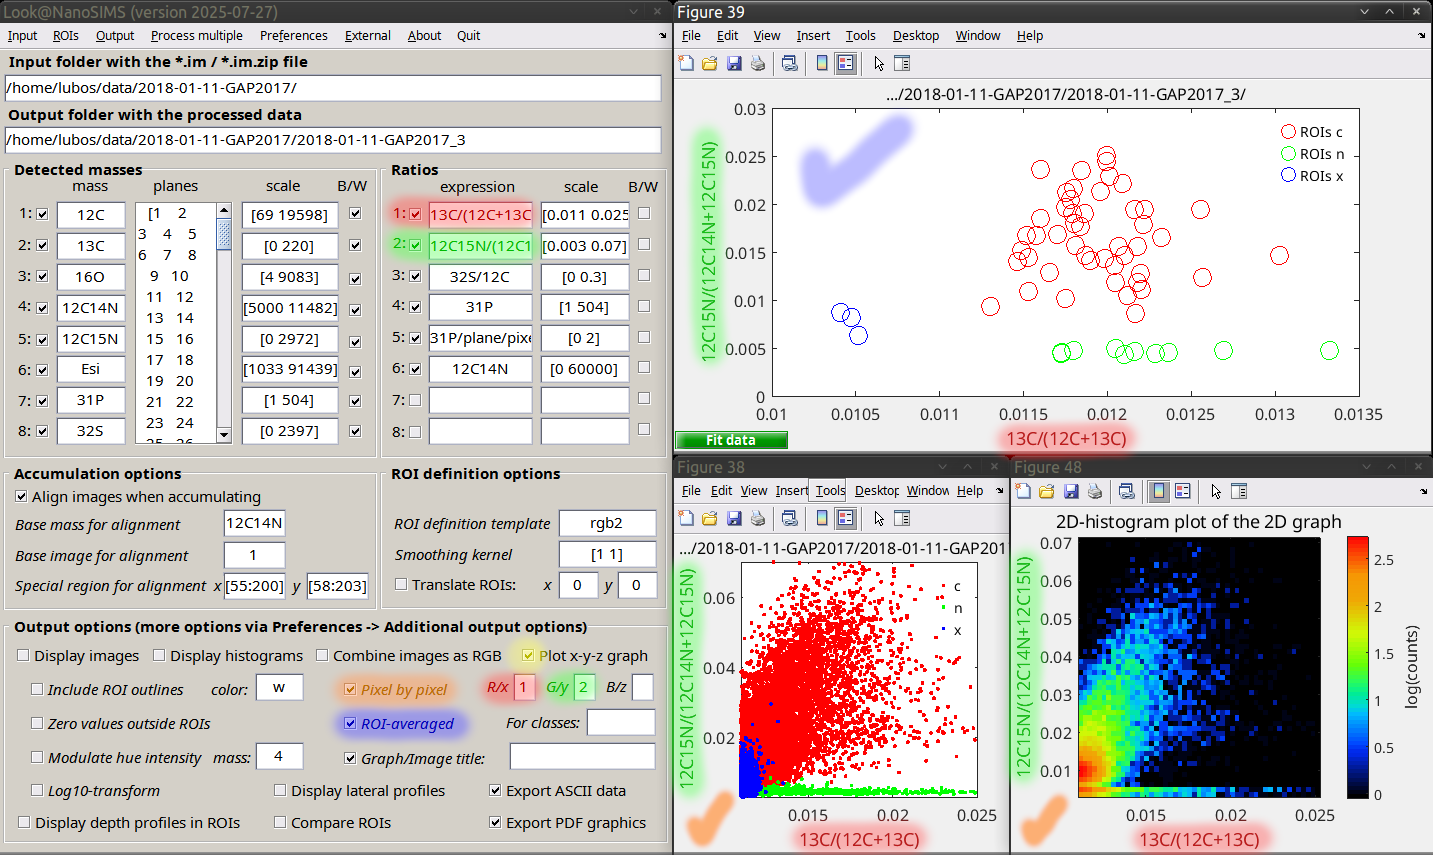
\includegraphics[width=0.9\textwidth]{figs3/LANS-scatter-plots}
\caption{\label{fig:scatter-plots}%
Examples of 2D scatter plots generated by LANS. They can show ROI-averaged values (blue) or pixel-by-pixel values (orange).}
\end{figure}
 
\nb{If all three fields are filled in, the ROI-specific values will be plotted in a~3D scatter plot (x--y--z). If only two of the three fields are filled in, a~2D scatter plot (x--y) will be created.}

\nnb{In the \ttt{Ratios} or \ttt{Detected masses} box, ensure that the checkboxes corresponding to the identifiers filled in the \lanstf{R/x}, \lanstf{G/y} and \lanstf{B/z} fields are checked, too. }

\s{Check \lanscb{ROI-averaged} or \lanscb{Pixel by pixel} (also in the \ttt{Output options} box; Fig.~\ref{fig:scatter-plots}) if you want to display a~scatter plot for ROI-specific or pixel-specific values, respectively.}

\nnb{You can have both of them checked at the same time. }

\s{Check \lanscb{Export ASCII data} and \lanscb{Export PDF graphics} to ensure that the data and graphs will be exported (in the \ttt{dat} and \ttt{pdf} sub-folders of the dataset folder, respectively).}

\s{When plotting scatter plots, it is typically not necessary anymore to display the corresponding images. If this is the case for you, uncheck the \lanscb{Display images} checkbox.}

\s{Select \lans{Output} $\ra$ \lans{Display masses} or \lans{Display ratios} to \bb{create scatter plots} of the ROI-specific or pixel-specific values of the desired quantities and \bb{export the values and graphs}. }

\nb{In the process, you will be prompted to select a~ROI classification file. If the file exists (and it is up-to-date), select it. In this case, different colors will be used to mark ROI from different classes (Fig.~\ref{fig:scatter-plots}).} 

\nnb{If the ROI classification file does not exist, click \ttt{Cancel} or press \ttt{Esc} when prompted for the file. In this case, all ROIs will be treated equally and displayed in one color.}

\nb{If you only want to display values for specific classes, you can enter the identifiers for those classes in the \lanstf{For classes} field (just below the R/x, G/y and B/z fields) first, then select \lans{Output} $\ra$ \lans{Display masses} or \lans{Display ratios}.}

\nb{If you choose to display ROI-specific values, it is possible to add a~ROI identifier and an~error-bar to each data point. This is achieved by selecting the corresponding options via \lans{Preferences} $\ra$ \lans{Additional output options}. The error-bar size will indicate the Poisson error, derived from the total ion counts per ROI.}

\nb{The output data and images will be stored in the \ttt{dat} and \ttt{pdf} sub-folders of the dataset folder, respectively. Formatting of the data output is self-explanatory based on the first two lines in the output file.}

\s{Select \lans{Output} $\ra$ \lans{Check output consistency} to check that the exported ROI-specific data are consistent with the defined ROI  classes (only relevant if working with classified ROIs). }

\nb{The output is consistent if the number of defined ROIs, the number of classified ROIs, and the number of ROIs for which the ROI-specific data have been exported, is the \emph{same}.}

\nnb{Output inconsistency can occur if, e.g., you redefine ROis but forget to reclassify them or reexport the ROI-specific data (or any combination of these three actions).}

\s{When prompted, select the ROI classification file and view the results of the consistency check in the Matlab console. }

\nnb{If any of the output lines does not contain \ttt{OK}, you should revise your analysis by reclassifying the ROIs or reexporting the ROI-specific data for the affected variables.}

%%

\subsection{Display depth profiles in ROIs}
\setcounter{step}{0}

\goldbox{}
NanoSIMS measurements are conducted by sputtering away the sample material in multiple scans over the same field of view while collecting the secondary ions. The resulting image stack therefore reflects elemental and isotopic distribution of the sample along the vertical dimension. You can display and export this vertical (depth) variation in ROIs using the following steps.
\tcbe

\sbx{Ensure that ROIs have been defined or loaded into the current LANS session.}

\s{Check \lanscb{Display depth profiles in ROIs} in the \ttt{Output options} box.}

\nnb{Typically, you will want to uncheck all other checkboxes in the \ttt{Output options} box to prevent cluttering of your screen with too many figures.}

\s{Check \lanscb{Detected masses} or \lanscb{Ratios} for which you want to display the depth profiles.}

\s{Select \lans{Output} $\ra$ \lans{Display masses} or \lans{Display ratios}.}

\s{Observe the output in the Matlab console, which informs you about significant trends with depth of the particular mass or ratio in ROIs.}

\nb{In the process, the depth profiles are exported in data files with an extension \ttt{dap} (located in the \ttt{dat} sub-folder of the dataset folder).}

\s{In the new window that opens, select ROI identifiers for which you want to display the depth profiles. Then, select the mass or ratio in the list to display the depth profiles in the selected ROIs (Fig.~\ref{fig:depth-profiles}).}

\begin{figure}[!ht]
\centering
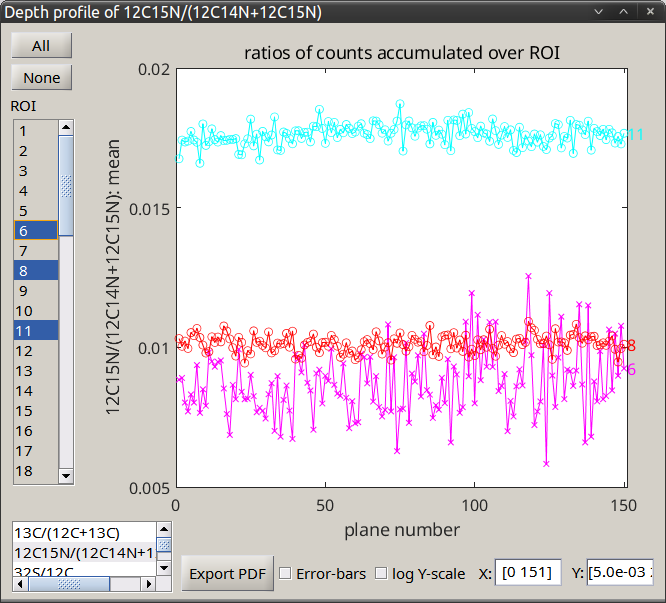
\includegraphics[scale=0.4]{figs3/LANS-depth-profiles}
\caption{\label{fig:depth-profiles}%
Using LANS to display depth profiles of ion counts and ion count ratios in ROIs.}
\end{figure}

\s{Select \lans{Export depth profile} to export the graph with depth profiles in the currently selected ROIs.}

%%

\subsection{Finalize the processing of an individual dataset}
\label{sec:final-steps}
\setcounter{step}{0}

\goldbox{}
If you want to reprocess a~particular dataset in the future and start the processing from the same stage where you finished, you will need to have the data processing settings stored. If you want to share or communicate the results with collaborators, a~graphical output where all the images and graphs generated by LANS are nicely assembled might be a~good idea. Finally, if you want to make a~backup of the processed data for yourself or for sharing with collaborators, having a~compressed version of the processed data folder would probably be the best approach. You can generate these types of output quickly within LANS using the following steps:
\tcbe

\s{Select \lans{Output} $\ra$ \lans{Generate LaTeX + PDF output} to export results of your analysis in a~PDF document (example shown in Fig.~\ref{fig:outputG}). }

\nb{Before you do this, select checkboxes in the \ttt{Output options} box to specify which kind of results you want to have included in the graphical output, such as  \lanscb{images}, \lanscb{scatter plots}, \lanscb{RGB overlays}, \lanscb{histograms}, \lanscb{depth profiles}, etc.}

\nb{If you check \lanscb{View PDF after export} (available via \lans{Preferences} $\ra$ \lans{Additional output options}) and correctly set the full path to a~PDF viewer in the \ttt{PDF\_VIEWER} variable (this variable is defined in the \ttt{lans\_paths.m} file), the PDF output will automatically be displayed after it has been generated. This can be convenient if you want to see the results quickly, without the need for browsing through the different folders on your computer.}

\begin{figure}[!ht]
\centering
\begin{tabular}{ccc}
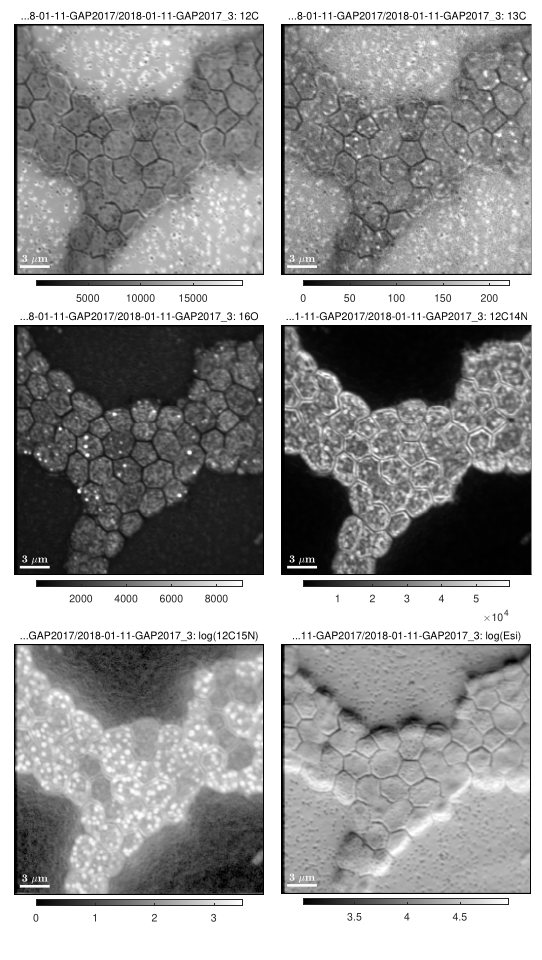
\includegraphics[width=0.31\textwidth, valign=t]{figs3/outputG1}
&
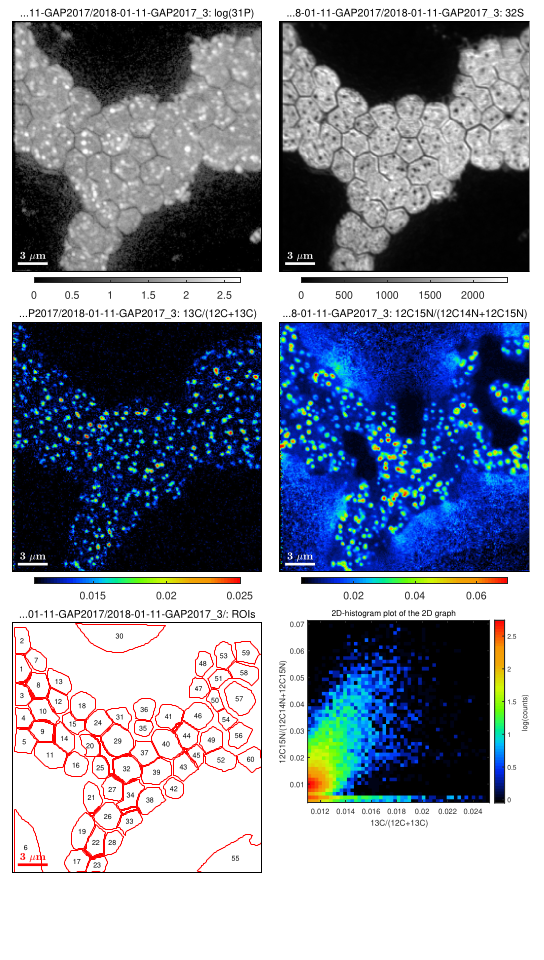
\includegraphics[width=0.31\textwidth, valign=t]{figs3/outputG2}
&
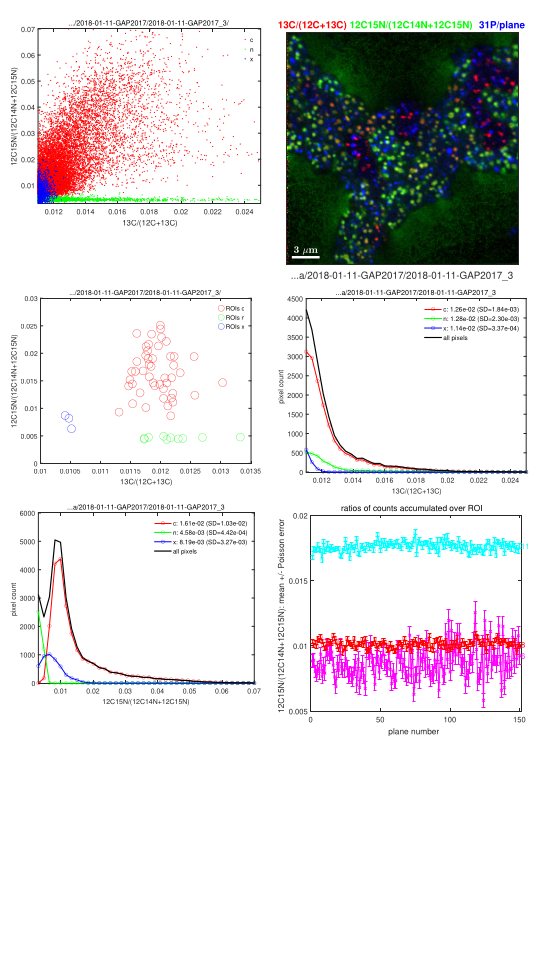
\includegraphics[width=0.31\textwidth, valign=t]{figs3/outputG3}
\end{tabular}
\caption{\label{fig:outputG}%
Example of the first three pages in the graphical output generated at the end of processing of an individual dataset with LANS.}
\end{figure}

\s{Select \lans{Preferences} $\ra$ \lans{Store preferences} to save the settings of the current data processing session in a file (it is recommended to use the file name \ttt{prefs.mat}). }

\nb{This is useful when you want to return to the analysis of the same file in the future, but also if you want to later combine results of your analyses of multiple datasets via ``metafile processing'', as described in Section~\ref{sec:level2}. Therefore, it is highly recommended that you do this for every processed dataset.}

\nnb{More specifically, the preferences file will contain all information for the currently processed dataset that you see in the main LANS window, including the names of detected masses, planes selected for alignment, formulas for ion count ratios, scales for mass and ratio images, output options, etc.}

\s{Select \lans{Preferences} $\ra$ \lans{Backup (full) folder with processed data}.}

\nbx{This will compress the \emph{entire} content of the processed data folder in a~\ttt{zip} file.}

\nnb{Additionally, a~copy of the PDF output file will be created and renamed to match the name of the processed data.}

\s{Alternatively, select \lans{Preferences} $\ra$ \lans{Backup (minimal) folder with processed data}.}

\nb{This will only compress the \emph{minimal} information in the processed data folder, based on which the rest of the processed data can easily and reproducibly be generated by repeating the processing steps in LANS. }

\nnb{This minimal information includes the preferences (e.g., \ttt{prefs.mat}), plane alignment information (\ttt{xyalign.mat}), ROI definition (e.g., \ttt{ROIs.mat}), and ROI classification (e.g., \ttt{ROIs.dat}).}
